% SMPC 2019 proceedings

% remember to compile twice in LaTeX, then with makeIndex, then with LaTeX again.


\documentclass[10pt, twoside, letter]{book}
%\usepackage{url}
\usepackage[utf8]{inputenc}
\usepackage[T1]{fontenc}
\usepackage{multicol}
\usepackage{setspace}
\usepackage{graphicx}
\usepackage{wrapfig}
\usepackage{mathptmx} 
\usepackage{fancyhdr}
\usepackage{makeidx}
\usepackage{pdfpages}
\usepackage{hyperref}
\usepackage{geometry}
\usepackage{tipa}
\usepackage{textcomp}
\usepackage[labelformat=empty]{caption}
\usepackage{array}
\usepackage{float}
\usepackage[section]{placeins}
\usepackage{helvet}

% formatting commands
% defining table dimensions for talks headings (AB) and poster headings  (DE) 
\newcolumntype{A}{>{\raggedleft\arraybackslash}m{1.7cm}}
\newcolumntype{B}{>{\raggedright\arraybackslash}b{14cm}}
\newcolumntype{D}{>{\raggedleft\arraybackslash}m{1cm}}
\newcolumntype{E}{>{\raggedright\arraybackslash}b{14cm}}

\renewcommand*\familydefault{\sfdefault}
\setlength{\intextsep}{5pt} 

\geometry{inner=2.5cm,outer=2.5cm,top=2.3cm,bottom=2.3cm}
\pagestyle{fancy}
\hypersetup{
    colorlinks=true,
    linkcolor=blue,
    filecolor=magenta,      
    urlcolor=cyan,
}
% fancy header details
\lhead[\thepage]{2019 Biennial Meeting of the Society of Music Perception and Cognition}
\rhead[August 5-7, 2019 in New York City, USA]{\thepage}
\lfoot{}
\cfoot{}

\makeindex
\usepackage[totoc]{idxlayout}

\includepdfset{offset=0mm 0}

\pdfinclusioncopyfonts 1


% The Document itself
\begin{document}
% cover
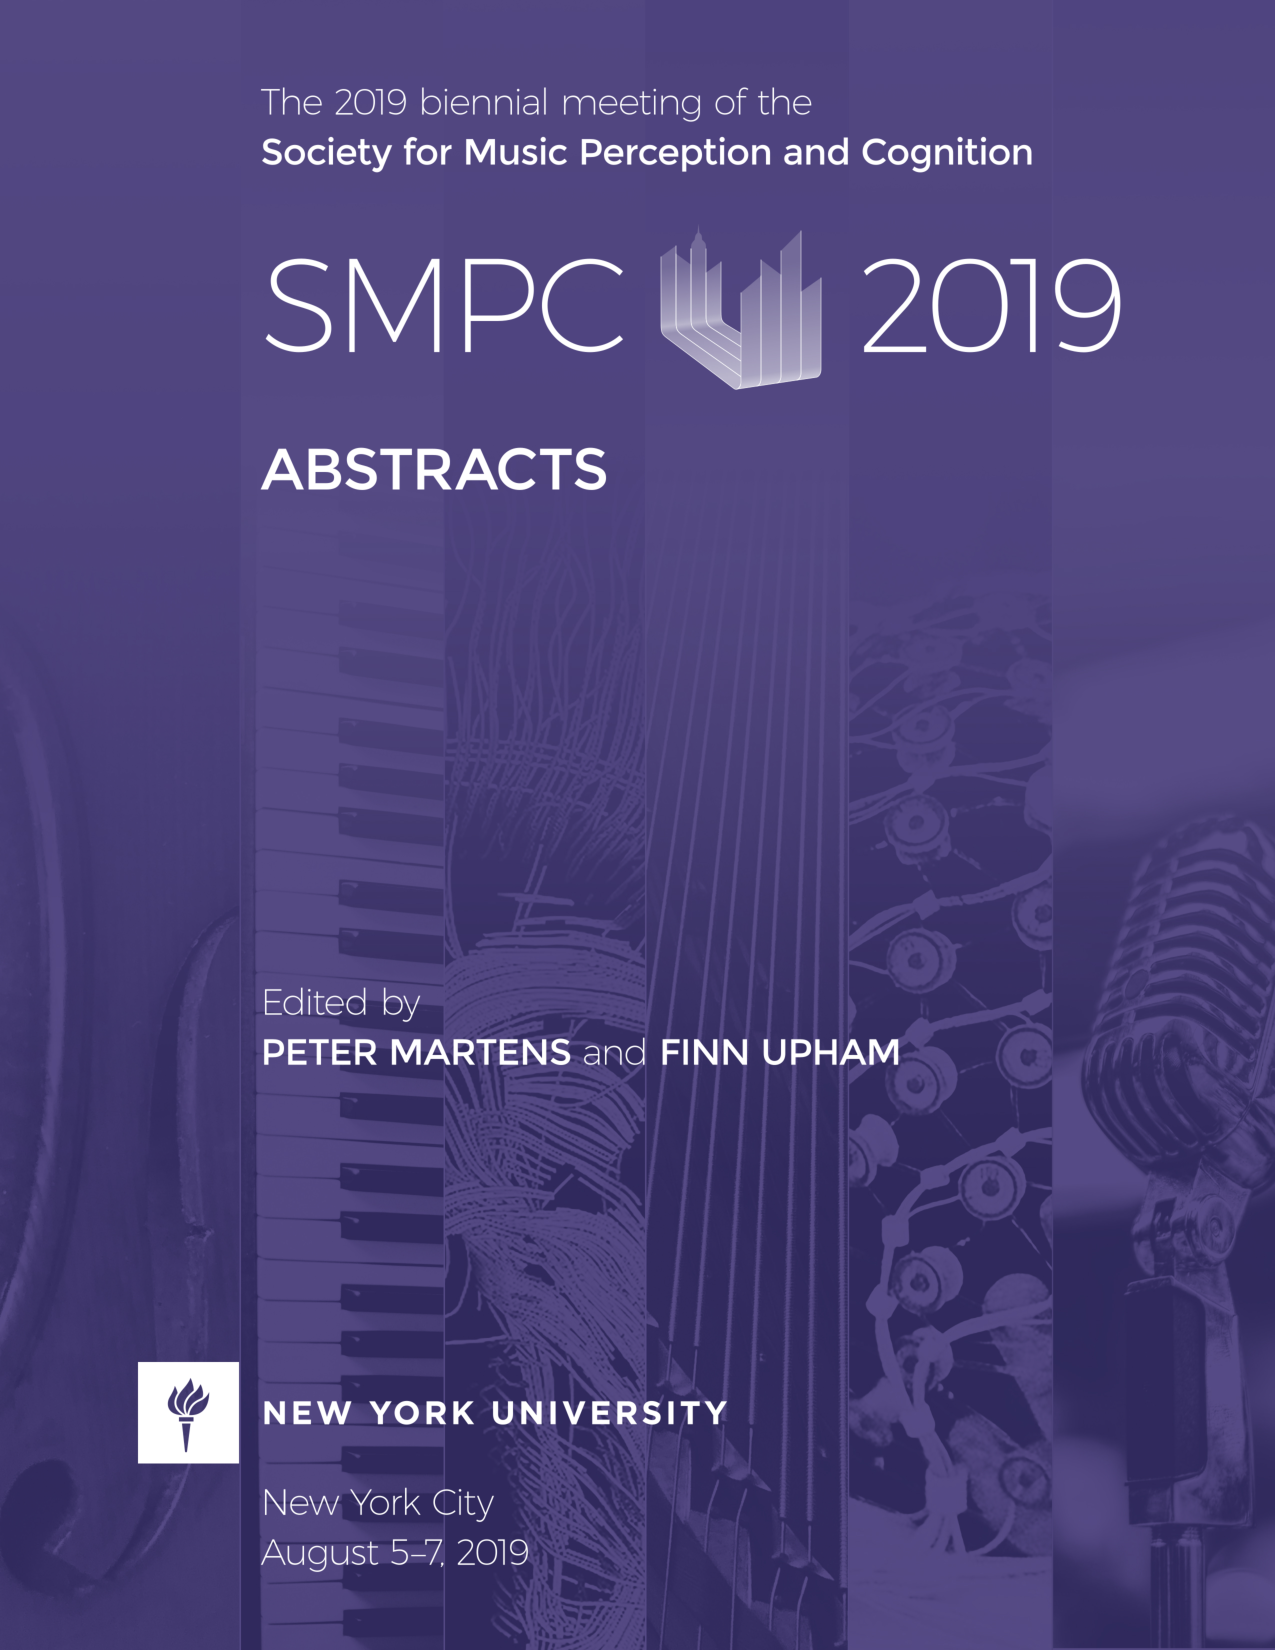
\includepdf[pages=1,pagecommand=\thispagestyle{empty}]{cover_Abs_2.pdf}%

\tableofcontents

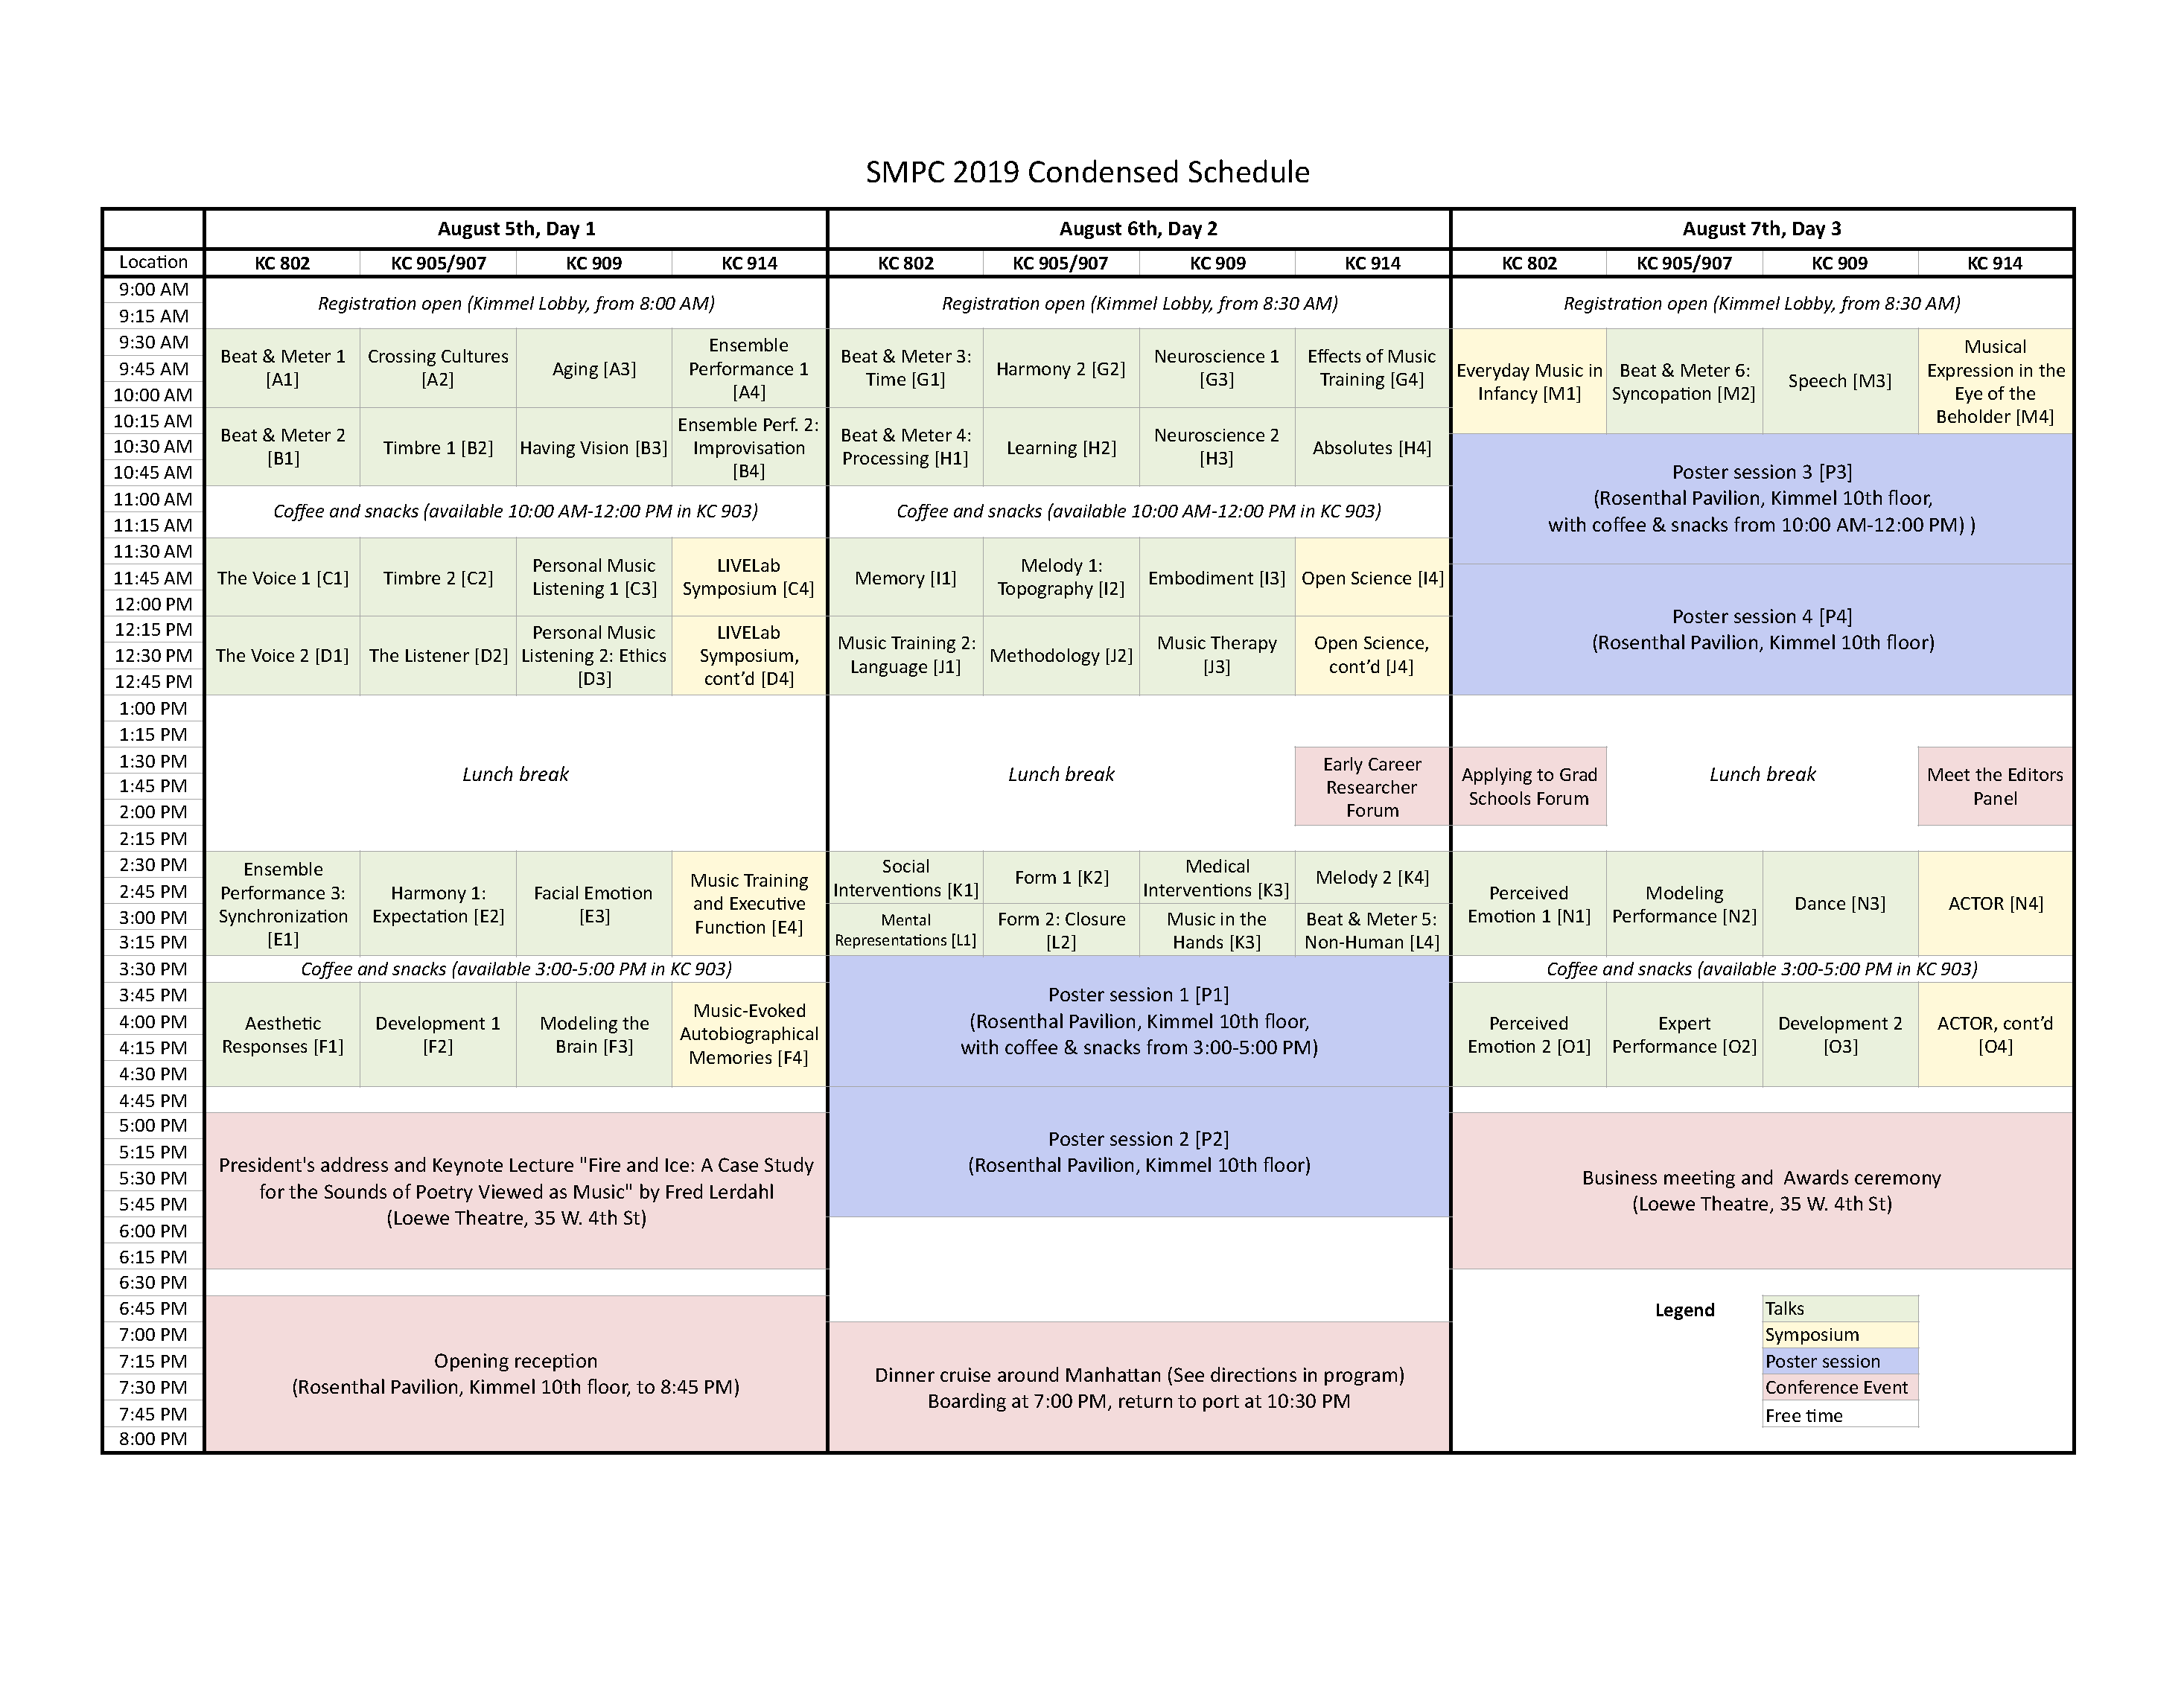
\includepdf[angle=90,pages=1,pagecommand=\thispagestyle{empty}]{SMPC2019_Condensed_colour.pdf}


%Abstracts, changing header along the way
\rhead[Talks on Day 1, August 5, 2019]{\thepage}
\input{Aug5_Talks_Abstract.tex}

\rhead[Talks on Day 2, August 6, 2019]{\thepage}
\input{Aug6_Talks_Abstract.tex}

\rhead[Posters on Day 2, August 6, 2019]{\thepage}
\input{Aug6_Poster_Abstract.tex}

\rhead[Talks on Day 3, August 7, 2019]{\thepage}
\input{Aug7_Talks_Abstract.tex}

\rhead[Posters on Day 3, August 7, 2019]{\thepage}
\input{Aug7_Poster_Abstract.tex}

\singlespacing
\printindex


\end{document}